\chapter{Quente e frio}\label{ch:g1:hot-and-cold}

A sopa solta fumacinha, o sorvete faz o dente doer e o banco do carro
no verão queima as pernas da gente. O quente e o frio estão em toda
parte. Neste capítulo aprendemos a compará-los, a descobrir o que
esquenta as coisas --- e a ver o que acontece com um cubo de gelo
quando o calor ganha a disputa.

\section{Mais quente e mais frio}

\begin{definition}[Quente e frio]\label{def:g1:hot-and-cold:words}
\emph{Quente}\index{quente} e \emph{frio}\index{frio} são palavras de
comparação, como grande e pequeno. A sopa é quente \emph{em relação
à} sua mão; o gelo é frio \emph{em relação à} sua mão. Entre os dois
há uma escada inteira de palavras: congelando, gelado, frio, morno,
quentinho, quente, escaldante.
\end{definition}

\begin{omfigure}
\begin{tikzpicture}[scale=0.85]
  \draw[-Stealth, very thick] (0,0) -- (11.2,0);
  \node[below, font=\small] at (0.6,-0.25) {cubo de gelo};
  \node[below, font=\small] at (3.2,-0.25) {água fria};
  \node[below, font=\small] at (5.7,-0.25) {minha mão};
  \node[below, font=\small] at (8.2,-0.25) {sopa quente};
  \node[below, font=\small] at (10.4,-0.25) {chama};
  \fill[omDef] (0.6,0) circle (2.6pt);
  \fill[omDef] (3.2,0) circle (2.6pt);
  \fill[omMeth] (5.7,0) circle (2.6pt);
  \fill[omThm] (8.2,0) circle (2.6pt);
  \fill[omThm] (10.4,0) circle (2.6pt);
  \node[above, font=\small] at (1.2,0.3) {mais frio};
  \node[above, font=\small] at (9.9,0.3) {mais quente};
\end{tikzpicture}

{\small Uma escada do frio ao quente: cada coisa acha o seu lugar, com
a sua mão em algum ponto do meio.}
\end{omfigure}

\begin{example}[Colocando três bebidas em ordem]\label{ex:g1:hot-and-cold:drinks}
Na mesa: um chocolate quente, um copo de água da torneira e um copo
de suco de laranja recém-tirado da geladeira. Do mais frio ao mais
quente: o suco, depois a água da torneira, depois o chocolate quente.
A água da torneira é fria ao lado do chocolate, mas quente ao lado do
suco --- as palavras de comparação sempre trabalham em dupla.
\end{example}

\begin{remark}[O tato se engana]\label{rem:g1:hot-and-cold:fooled}
Lembre das três tigelas do capítulo passado: a mesma água morna
pareceu quente para uma das mãos e fria para a outra. E toque numa
colher de metal e numa colher de pau que passaram a noite inteira na
mesma cozinha: a de metal \emph{parece} mais fria, embora nada na
cozinha esteja mais frio do que o resto. O tato é um guarda útil, mas
não é um juiz justo --- um dia desses vamos precisar de um
instrumento que não se deixa enganar: o termômetro, que chega num
capítulo mais adiante.
\end{remark}

\begin{method}[Comparar quente e frio com justiça]\label{met:g1:hot-and-cold:compare}
Para decidir qual de duas tigelas de água está mais quente:
\begin{enumerate}
  \item use a \emph{mesma} mão nas duas --- duas mãos podem discordar;
  \item toque numa e logo em seguida na outra --- esperar deixa as
        coisas mudarem;
  \item para ter mais certeza ainda, peça a um colega que também
        experimente, sem contar antes a sua resposta.
\end{enumerate}
Se você e o seu colega concordarem, a observação é firme.
\end{method}

\section{O que esquenta as coisas}

\begin{example}[Aquecedores]\label{ex:g1:hot-and-cold:warmers}
Algumas coisas esquentam tudo o que está por perto: o Sol esquenta o
banco da praça, a chama esquenta a panela, o aquecedor esquenta a
sala e o seu próprio corpo esquenta o cobertor. Até esfregar
esquenta: junte as palmas das mãos e esfregue depressa enquanto conta
até $10$ --- sinta elas esquentarem.
\end{example}

\begin{omfigure}
\begin{tikzpicture}[scale=0.8]
  % the sun, high on the left
  \fill[omThm] (1.0,3.3) circle (0.5);
  \foreach \a in {0,30,...,330} {
    \draw[omThm, thick] (1.0,3.3) ++(\a:0.68) -- ++(\a:0.32);
  }
  % ground line
  \draw[thick] (2.6,0) -- (11.6,0);
  % sunny bench, with two sun rays reaching it
  \draw[omThm] (1.55,2.95) -- (4.3,0.75);
  \draw[omThm] (1.75,3.1) -- (5.7,0.75);
  \draw[thick] (3.6,0.55) -- (6.4,0.55);
  \draw[thick] (3.8,0.55) -- (3.8,0) (6.2,0.55) -- (6.2,0);
  \node[below, font=\small] at (5.0,-0.15) {banco no sol: quente};
  % tree whose shade covers the second bench
  \draw[thick, fill=omExo!60] (8.05,0) rectangle (8.35,1.5);
  \draw[thick, fill=omMeth!45] (8.2,2.15) circle (0.95);
  \fill[omExo, opacity=0.3] (9.8,0.06) ellipse (1.75 and 0.2);
  \draw[thick] (8.6,0.55) -- (11.2,0.55);
  \draw[thick] (8.8,0.55) -- (8.8,0) (11.0,0.55) -- (11.0,0);
  \node[below, font=\small] at (9.9,-0.15) {banco na sombra: fresco};
\end{tikzpicture}

{\small Dois bancos na mesma praça, no mesmo dia. Aquele em que o Sol
bate está mais quente --- experimente com a mão num dia de sol.}
\end{omfigure}

\begin{example}[Experimente: sol e sombra]\label{ex:g1:hot-and-cold:sunshade}
Num dia de sol, ponha uma das mãos numa parede que está no sol e a
outra na mesma parede, na sombra. Mesma parede, mesmo dia --- mas o
lado ensolarado está claramente mais quente. O Sol é o grande
aquecedor de tudo o que está ao ar livre; daqui a pouco ele ganha um
capítulo inteiro só para ele.
\end{example}

\begin{remark}[O casaco não fabrica calor]\label{rem:g1:hot-and-cold:coat}
Um casaco não esquenta você do jeito que um aquecedor esquenta. É o
seu \emph{corpo} que fabrica o calor; o casaco só impede que esse
calor escape, como uma tampa sobre a sopa. É por isso que um casaco
largado sozinho numa cadeira fica frio por dentro --- não há nada
dentro dele fabricando calor para guardar.
\end{remark}

\section{Quando o calor ganha: o gelo derrete}

\begin{example}[A vida de um cubo de gelo]\label{ex:g1:hot-and-cold:icecube}
Ponha um cubo de gelo num prato, na cozinha. Ele está duro e frio. O
ar quente da sala vai esquentando o cubo pouco a pouco: ele fica cada
vez menor, uma poça cresce em volta dele e, depois de um tempo, só
sobra água. O calor da sala transformou gelo duro em água líquida ---
dizemos que o gelo \emph{derreteu}.
\end{example}

\begin{omfigure}
\begin{tikzpicture}[scale=0.8]
  % stage 1: a crisp cube, straight from the freezer
  \draw[thick] (0,0) -- (2.4,0);
  \draw[thick, omDef, fill=omDef!15] (0.85,0.02) rectangle (1.55,0.72);
  \draw[thick, omDef, fill=omDef!30]
    (0.85,0.72) -- (1.05,0.9) -- (1.75,0.9) -- (1.55,0.72) -- cycle;
  \draw[thick, omDef, fill=omDef!40]
    (1.55,0.02) -- (1.75,0.2) -- (1.75,0.9) -- (1.55,0.72) -- cycle;
  \draw[omDef!60] (0.93,0.6) -- (0.93,0.4);
  \node[below, font=\small] at (1.2,-0.22) {recém-saído do congelador};
  % stage 2: a smaller, rounding cube sitting in its own puddle
  \draw[thick] (4.4,0) -- (6.8,0);
  \draw[omDef, fill=omDef!25] (5.6,0.06) ellipse (0.75 and 0.11);
  \draw[thick, omDef, fill=omDef!15, rounded corners=1.6pt]
    (5.35,0.1) rectangle (5.8,0.55);
  \draw[thick, omDef, fill=omDef!30, rounded corners=1.2pt]
    (5.35,0.55) -- (5.49,0.67) -- (5.94,0.67) -- (5.8,0.55) -- cycle;
  \draw[thick, omDef, fill=omDef!40, rounded corners=1.2pt]
    (5.8,0.1) -- (5.94,0.22) -- (5.94,0.67) -- (5.8,0.55) -- cycle;
  \fill[omDef!60] (5.99,0.3) circle (0.045);
  \fill[omDef!60] (6.07,0.14) circle (0.035);
  \node[below, font=\small] at (5.6,-0.22) {um pouco depois};
  % stage 3: nothing left but water
  \draw[thick] (8.8,0) -- (11.2,0);
  \draw[omDef, fill=omDef!25] (10.0,0.06) ellipse (0.95 and 0.13);
  \draw[omDef!60] (9.5,0.1) .. controls (9.8,0.16) .. (10.15,0.12);
  \node[below, font=\small] at (10.0,-0.22) {o calor ganhou};
\end{tikzpicture}

{\small O mesmo cubo de gelo três vezes: a sala quente o derrete até
virar uma poça de água.}
\end{omfigure}

\begin{omfigure}
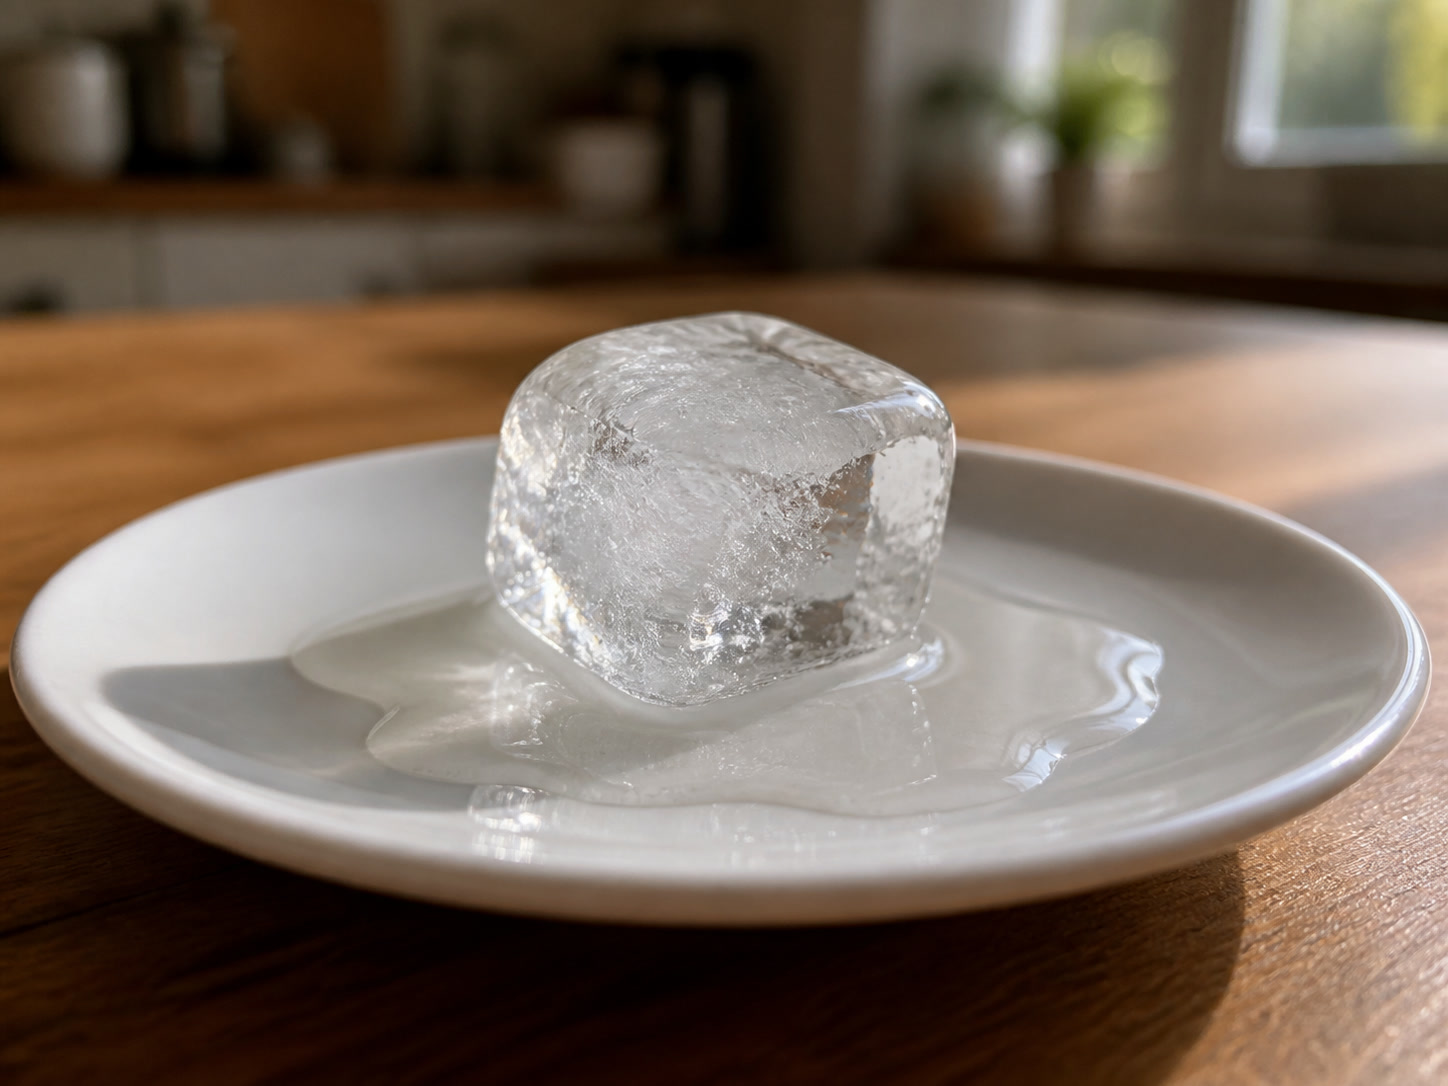
\includegraphics[width=0.52\linewidth]{images/book1/ai/g1-hot-cold-melting-cube.jpg}

{\small O calor trabalhando: o cubo de gelo da cozinha, flagrado no momento em que começa a derreter na própria poça.}
\end{omfigure}

\begin{example}[O frio também pode ganhar]\label{ex:g1:hot-and-cold:freezer}
O congelador faz o trabalho contrário: ponha um copinho de água lá
dentro à noite e de manhã você vai encontrá-la dura como pedra ---
gelo. O calor derrete o gelo e vira água; o frio forte transforma a
água de volta em gelo. A água vai continuar indo e voltando assim ao
longo de todo o livro.
\end{example}

\section{Exercícios}

\begin{exercise}[$\star$]\label{exo:g1:hot-and-cold:1}
Coloque em ordem, do mais frio ao mais quente: a água do banho; \ um
cubo de gelo; \ a sopa recém-tirada da panela; \ o ar do seu quarto.
\end{exercise}

\begin{exercise}[$\star$]\label{exo:g1:hot-and-cold:2}
Complete com a palavra de comparação: a água da torneira é \dots\ em
relação ao chocolate quente, mas \dots\ em relação ao suco de laranja
da geladeira.
\end{exercise}

\begin{exercise}[$\star$]\label{exo:g1:hot-and-cold:3}
Diga quatro coisas que esquentam o que está por perto. Qual delas
esquenta a praça inteira?
\end{exercise}

\begin{exercise}[$\star$]\label{exo:g1:hot-and-cold:4}
Esfregue depressa as palmas das mãos enquanto conta até $10$ e depois
encoste-as no rosto. O que você sente? O que a esfregação fez?
\end{exercise}

\begin{exercise}[$\star$]\label{exo:g1:hot-and-cold:5}
Dois cubos de gelo saem juntos do congelador. Um vai para um prato no
sol, o outro para um prato na sombra. Qual derrete primeiro, e por
quê?
\end{exercise}

\begin{exercise}[$\star$]\label{exo:g1:hot-and-cold:6}
O que tem na poça que fica no prato depois que o cubo de gelo
derrete? Para onde foi o gelo duro?
\end{exercise}

\begin{exercise}[$\star$]\label{exo:g1:hot-and-cold:7}
Um escorregador de metal e um banco de madeira passaram a manhã
inteira na sombra. Tom toca nos dois e diz que o escorregador está
mais frio. Use a \cref{rem:g1:hot-and-cold:fooled} para explicar o
que está acontecendo de verdade.
\end{exercise}

\begin{exercise}[$\star$]\label{exo:g1:hot-and-cold:8}
Usando o \cref{met:g1:hot-and-cold:compare}, explique como descobrir
qual de duas tigelas de água está mais quente. Por que você deve usar
a mesma mão nas duas?
\end{exercise}

\begin{exercise}[$\star\star$]\label{exo:g1:hot-and-cold:9}
Lea faz um boneco de neve e, com pena dele, enrola-o no seu casaco
quentinho. O irmão dela diz que o casaco vai derreter o boneco mais
depressa. Lea diz que o casaco vai mantê-lo frio por mais tempo. Quem
está certo, e por quê? (Pense na \cref{rem:g1:hot-and-cold:coat}: o
que um casaco faz de verdade?)
\end{exercise}
